\chapter{Θέμα 1}
\label{ch:exc1}
Στο θέμα 1 έπρεπε να ελαχιστοποιήσουμε την $f$ χρησιμοποιώντας την μέθοδο Μέγιστης Καθόδου που υλοποιήσαμε στο δεύτερο παραδοτέο. Η ελαχιστοποίηση έπρεπε να γίνει με ακρίβεια $e = 0.001$ για κάθε ένα από τα παρακάτω βήματα $\gamma$:
\begin{itemize}
    \item $\gamma = 0.1$
    \item $\gamma = 0.3$
    \item $\gamma = 3$
    \item $\gamma = 5$
\end{itemize}
Το αρχικό σημείο που επιλέχθηκε ήταν το $(-4, 7)$.
\sep
Για $\gamma = 0.1$:\newline
Η μέθοδος βρήκε ελάχιστο το $0$ στο σημείο $(-0.001, 0)$ έπειτα από 116 επαναλήψεις.
\begin{figure}[!h]
    \centering
    \subfloat[Convergence in 1D space]{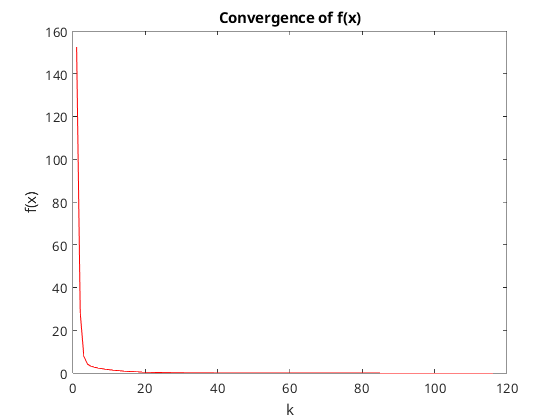
\includegraphics[width=0.5\textwidth]{Figs/1_conv_01.png}}
    \hfill
    \subfloat[Convergence in 2D space]{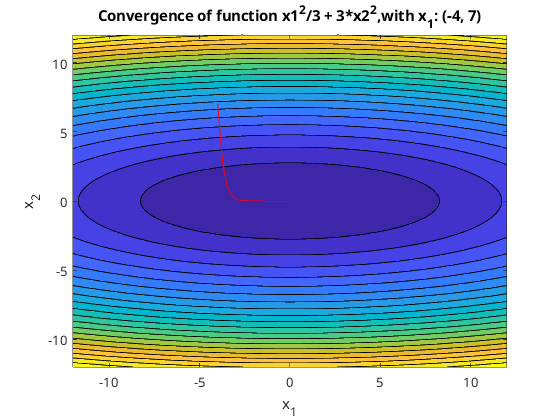
\includegraphics[width=0.5\textwidth]{Figs/1_01.png}}
\end{figure}
\sep
Για $\gamma = 0.3$:\newline
Η μέθοδος βρήκε ελάχιστο το $0$ στο σημείο $(0, 0)$ έπειτα από 49 επαναλήψεις.
\begin{figure}[!h]
    \centering
    \subfloat[Convergence in 1D space]{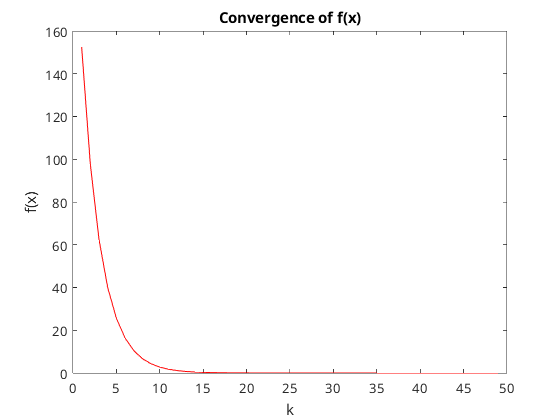
\includegraphics[width=0.5\textwidth]{Figs/1_conv_03.png}}
    \hfill
    \subfloat[Convergence in 2D space]{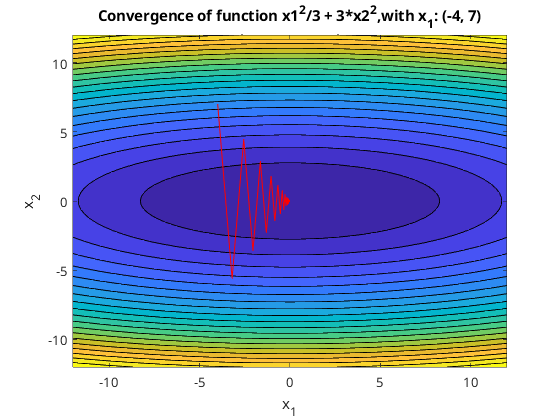
\includegraphics[width=0.5\textwidth]{Figs/1_03.png}}
\end{figure}
\sep
Για $\gamma = 3$:\newline
Όπως ήταν αναμενόμενο από την ανάλυση που έγινε στο \cref{sec:convergence} η μέθοδος δεν συνέκλινε.
Η τιμή του $x$ απομακρύνθηκε από το $(0, 0)$ και η μέθοδος τερμάτισε λόγω μίας συνθήκης που προστέθηκε στον κώδικα για να αποτρέψει το $x$ από το να απομακρυνθεί αρκετά από το σημείο ελαχίστου που είχε παρατηρηθεί αρχικά
\begin{figure}[!h]
    \centering
    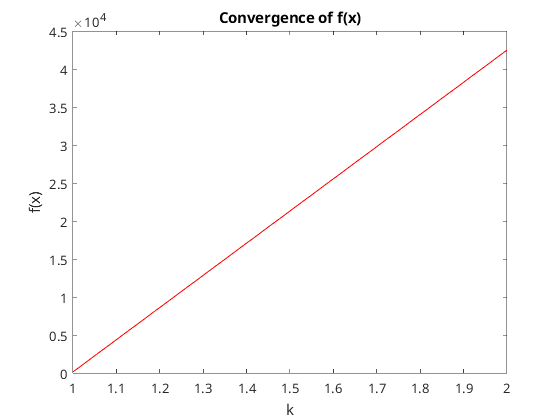
\includegraphics[width=0.7\linewidth]{Figs/conv_1_3.png}
    \caption{Η μεταβολή του $f(x_k)$ για $\gamma = 3$}
    \label{fig:1_3}
\end{figure}
\sep
Για $\gamma = 5$:\newline
Παρατηρήθηκαν παρόμοια αποτελέσματα όπως και στην παραπάνω περίπτωση.
\begin{figure}[ht]
    \centering
    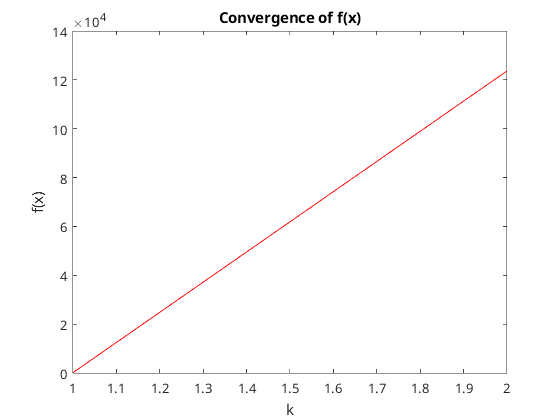
\includegraphics[width=0.7\linewidth]{Figs/conv_1_5.png}
    \caption{Η μεταβολή του $f(x_k)$ για $\gamma = 5$}
    \label{fig:1_5}
\end{figure}
